% Generated by paper_assets. Rebuild: python paper-artifacts/build.py fig1_rank_composition
% Figure drawn at the exact \textwidth; include without rescaling.
\begin{figure*}[t]
\centering
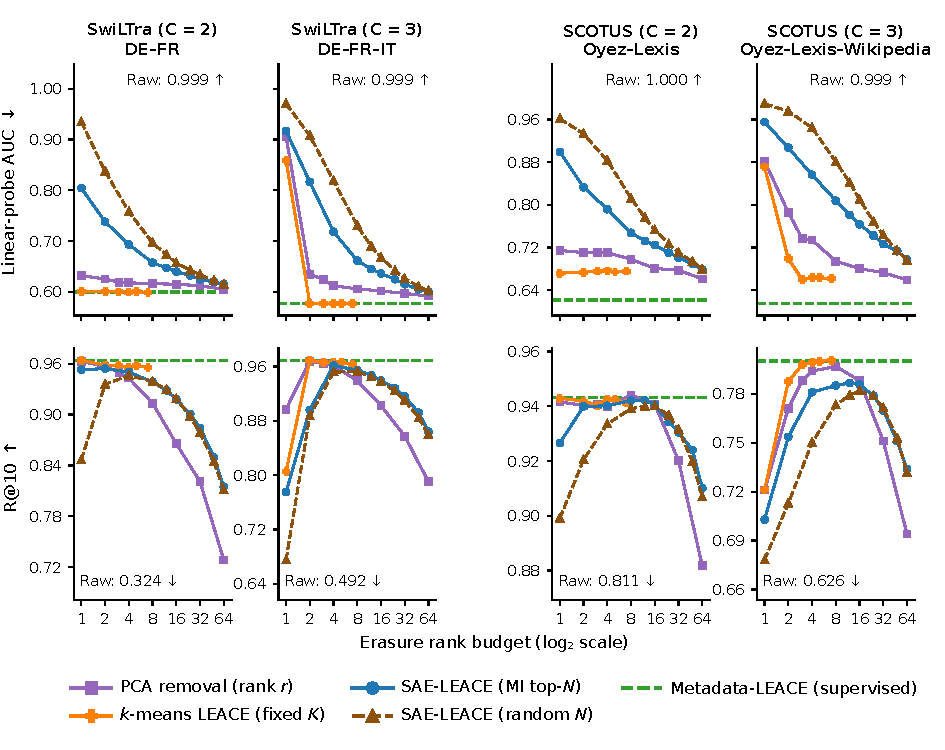
\includegraphics[width=\textwidth]{paper-artifacts/figures/fig1_rank_composition.pdf}
\caption{Erasure rank across binary and three-class compositions (E5-small). Top: held-out linear-probe nuisance AUC; bottom: R@10. The $x$-axis is the erasure rank budget on a $\log_2$ scale: $r$ principal directions for PCA removal, $K-1$ for $k$-means LEACE with $K$ fixed groups, and $N$ latent directions for SAE-LEACE, selected by MI or uniformly at random from the same SAE's latents that MI scores (training firing rate in $[0.02, 0.98]$; same operator). Each random point averages five draws per seed, so the random curve removes the selection signal. It is a nominal (maximum) rank, not a measured effective rank, and equal budgets do not imply equal removed variance. Points are means over seeds 0--4 of the coverage experiment (the random curve: a rerun on its splits and SAEs); seed SDs are not drawn and are given, with every per-seed value, in the accompanying data (they are largest for SAE-LEACE at small $N$, up to 0.15 in R@10). Metadata-LEACE (dashed) and Raw come from the same seeds. Raw is not drawn; its value is printed in each panel, the arrow showing that it lies above (AUC) or below (R@10) every curve of that panel. The two AUC panels of each corpus share a $y$-axis; each R@10 panel has its own. Only evaluated configurations are plotted, and lines only connect them.}
\label{fig:rank-composition}
\end{figure*}
